\section{Exercise}  %Jonathan / b-j8518 /Jul 19
\subsection{Problem 6 (Homework 3)} 
For $\phi \in {\rm DNN}_l$, $\phi$ is a continuous and piecewise linear function. $\mathbb{R}^d = \bigcup_i \bar{D}_i$, $D_i$ is a polyhedron. $\phi$ is linear on $D_i$. Plot some of these functions for $d=2$.

A neural network with ReLU activation functions produces a piecewise linear functions:
$NN(x,\theta)$ is piecewise in $x$.
Why is this a piecewise linear function? 
\begin{equation}\label{eq:DNN}
NN(x,\theta) = W_l \sigma (\cdots W_3 \sigma(W_2 \sigma (W_1 x+b_1) +b_2)+b_3 \cdots)+b_l
\end{equation}
Notice that
\begin{itemize}
\item linear map is piecewise linear,
\item and ReLU function is piecewise linear.
\item Composition of piecewise linear functions are piecewise linear. (Not trivial)
\end{itemize}
You should convince you self the third result is true. Being piecewise linear is the same thing that Hessian is zero or almost everywhere. 
The whole point of this exercise is to study the piecewise linear functions which are results from neural network process \eqref{eq:DNN}. 

For example, Consider the grid as follows.
\begin{figure} [H]%\label{mugrid-bi}
\begin{center}
\setlength{\unitlength}{0.445mm}
\begin{picture}(40,40)(40,0)
\linethickness{0.1mm}
\multiput(0,40)(15,0){3}{\line(0,-1){30}}
\multiput(0,10)(0,15){3}{\line(1,0){30}}
\put(0,10){\line(1,1){30}}
\put(15,10){\line(1,1){15}}
\put(0,25){\line(1,1){15}}
\end{picture}
\end{center}
\end{figure}
And consider functions that piecewise linear on each triangles.
In finite element, we consider piecewise linear functions which are linear on a `nice' set of polygon that tile the plane. 
Now we show how to implement it. There is a network we will plot.
\begin{python}
import torch
import torch.nn as nn
from torch.autograd import Variable
import matplotlib as plt

import numpy as np


class TestNet(nn.Module):
	def __init__(self):
		super(TestNet, self):__init__()
		self.function = nn.Sequential(nn.Linear(2, 25), nn.ReLU(), nn.Linear(25, 25), nn.ReLU(), nn.Linear(25, 1))
	def forward(self, x):
		return self.finction(x)
		
def main():
	net = TestNet()
	dy = 0.05
	dx = 0.05
	size = 400
	df_x = torch.zeros(size, size)
	df_y = torch.zeros(size, size)
	for i in range(size):
		for i in range(size)
			q = Variable(torch.Tensor([-1 + (i + 0.5) * dx, -1 + (j + 0.5) * dy]), requires_grad=True)
			output = net(q)
			df = torch.autograd.grad(output, q)
			df_x[i, j] = df[0][0]
			df_y[i, j] = df[0][1]
		df_x = (df_x - torch.min(df_x)) / (torch.max(df_x) - torch.min(df_x))
		df_y = (df_y - torch.min(df_y)) / (torch.max(df_y) - torch.min(df_y))
		df_color = torch.zeros(size, size, 3)
		df_color[:, :, 0] = df_x
		df_color[:, :, 1] = df_y
		plt.imshow(df_color)
		locs._labels = plt.xticks()
		locs = locs[1:]
		new_labels = []
		for i in locs:
			new_labels.append(-1.0 + i * dx)
		plt.xticks(locs, new_labels)
		plt.yticks(locs, new_labels)
		plt.show()
\end{python}

\subsection{Tips for Final Project} %Jonathan / b-j8526 /Jul 
In this section, we will introduce some tools that might be used in the final project. PyTorch has a library here call \emph{torchvision.models}. PyTorch also implement all of the model in the list for you, so you don't need to build it yourselves.
\begin{itemize}
\item AlexNet
\item VGG
\item ResNet
\item SqueezeNet
\item DenseNet
\item Inception v3
\item GoogLeNet
\item ShuffleNet v2
\item MobileNet v2
\item ResNeXt
\item Wide ResNet
\item MNASNet
\end{itemize}
However, all of the models implemented here are built for ImageNet, which is a dataset consisting much bigger images than CIFAR10. 

For example, if we look at one of the models, the VGG16 model. You can create a model:
\begin{python}
import torchvision.models as models
model = models.vgg16()
\end{python}
You can use \emph{print(model)} to see the list of the layers implemented.
\begin{figure}
\begin{center}
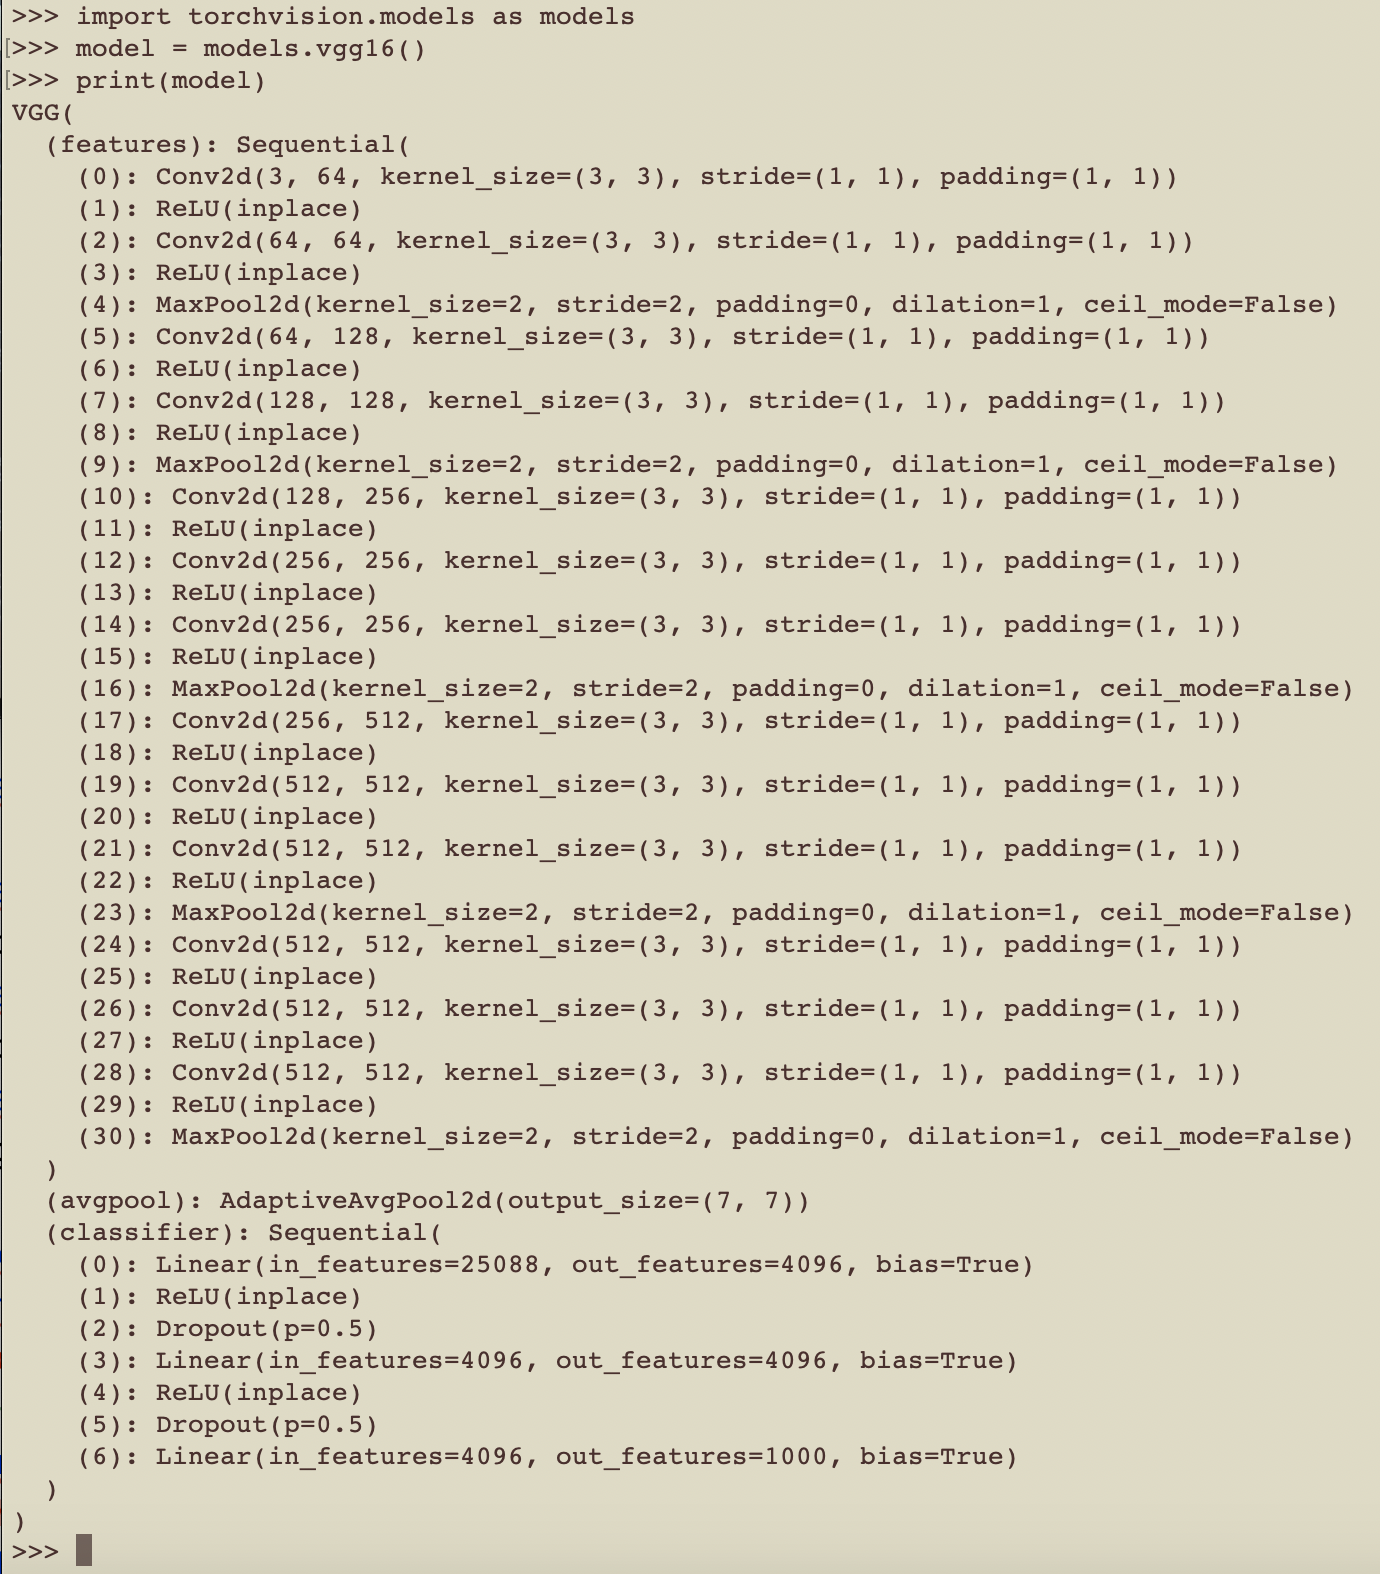
\includegraphics[scale=0.5]{../figures/497Proj_vgg16}
\end{center}
\end{figure}
You may notice that this is pretty deep, and there is a lot of max pooling layers. Each of max pooling step will decrease the size of the image by factor 2. If you plug in the CIFAR10
image which is $32\times 32$, then after a couple of these max pooling, it will be a single pixel. So the point is the model is too deep for CIFAR10. Because this model is implemented for ImageNet and too big, you can just take the model and implement it. But it's better to use this model as a template for VGG and make it smaller for CIFAR10. Use fewer channels in each convolution and use fewer layers.

The other model is the ResNet model. We can print the list of the layers in ResNet in the same way. 
This is a bit more complicated and also written for ImageNet. You should reduce number of channels and number of layers, and keep the same structure.



